\chapter{\scshape CVMix Parameterizations}
\label{chapter:cvmix_intro}

\minitoc
\vspace{.5cm}

We provide here an overview to the various parameterized vertical
mixing schemes available with Community Ocean Vertical Mixing
(CVMix) Parameterizations.  


\section{Vertical mixing parameterizations in CVMix}
\label{section:vert_mix_schemes_cvmix}

The CVMix Project aims to address the needs of various ocean modeling
groups to code, test, tune, and document parameterizations of oceanic
vertical mixing for numerical ocean simulations.  The project focuses
on first-order turbulence closures for vertical mixing
processes.\footnote{Those interested in higher order turbulence
  closure schemes for oceanm odeling may find the General Ocean
  Turbulence Model (GOTM) from \cite{GOTM} to be suitable.}  CVMix
does {\it not} determine time stepping for the model prognostic
fields.  Instead, time stepping is the responsibility of the calling
model code.  The following schemes are targets for the CVMix
parameterizations during phase I of the development.

\begin{itemize}

\item {\sc Static background mixing} (Chapter
  \ref{chapter:cvmix_background}): Certain turbulent processes, in
  particular the ambient background gravity wave ``noise'', constitute
  a background level of mixing that is largely steady in time from the
  pespective of large-scaling ocean modeling.  Though assumed to be
  time independent, these processes generally have a nontrivial space
  dependence.  CVMix provides options for various of these time
  independent schemes:
\begin{itemize}
\item the vertical profile from \cite{BryanLewis1979};
\item the profile from \cite{Henyey_etal1986} in which mixing near the
  equator is very small, as measured by \cite{Gregg_etal2003}; 
\item the approaches from \cite{Jochum2009}, in which enhanced mixing
  from parametric subharmonic mixing is included. 
\end{itemize}


\item {\sc Shear induced mixing} (Chapter \ref{chapter:cvmix_shear}):
  The following schemes are available for shear mixing:
 \begin{itemize}
 \item \cite{PPvmix}, applicable largely for tropical circulation;
 \item \cite{LargeKPP} and \cite{Large_Gent1999}, which builds on the
   \cite{PPvmix} scheme;
 \item \cite{Jacksonetal2008}, which employs a vertically non-local
   method to determine shear mixing throughout the World Ocean.
 \end{itemize}


\item {\sc Tidally induced mixing} (Chapter
  \ref{chapter:cvmix_tidal}): The following schemes are available for
  parameterizing mixing induced by ocean tides.
  \begin{itemize}
   \item \cite{Simmonsetal2004} 
   \item \cite{Melet_etal_2013}
   \item  the bottom boundary mixing scheme from \cite{Legg_eta2006},
     including bottom mixing from barotropic tides. 
\end{itemize}


\item {\sc Double diffusive processes} (Chapter
  \ref{chapter:cvmix_ddiffusion}): Double diffusive processes arise
  from the distinct mixing properties of temperature and
  salinity. 

\item {\sc KPP surface boundary layer} (Chapter
  \ref{chapter:cvmix_kpp}): The K-profile parameterization (KPP)
  scheme from \cite{LargeKPP} provides for a diffusivity as well as a
  non-local transport, each within the surface planetary boundary
  layer.

\item {\sc Vertical convective mixing}: Vertical profiles can become
  gravitationally unstable, such as when the ocean is forced with a
  negative buoyancy flux.  Older approaches such as \cite{CoxModel}
  and \cite{Rahmstorf1993} considered a convective {\it adjustment}
  algorithm, in which vertical pairs of grid cells were adjusted
  towards a profile of static stability.  In effect, the vertical
  diffusivity is infinite when using adjustment schemes.  CVMix does
  {\it not} provide options for convective adjustment.  Instead, CVMix
  allows for the specification of a diffusivity that is large in
  regions of gravitational instability, thus enabling vertical
  convective {\it mixing} rather than {\it adjustment}.  Notably, when
  using the KPP surface boundary layer scheme, convective mixing is
  {\it not} computed inside the KPP boundary layer.  Instead, it is
  only computed beneath the boundary layer, and it is done so {\it
    after} the KPP boundary layer matching has occurred (see Section
  \ref{section:vert_mix_schemes_ordering_cvmix}).


\end{itemize}


\section{The general form of CVMix parameterizations}
\label{section:vert_mix_schemes_general_cvmix}

All schemes considered in CVMix can be formulated in terms of a
diffusivity and a non-local transport.  That is, the vertical
turbulent flux of a scalar or velocity component is written in the
form
\begin{equation}
  \overline{w' \, \lambda'} = 
  -K_{\lambda} \left( \frac{\partial \overline{\lambda}}{\partial z} - \gamma_{\lambda} \right),
\label{eq:cvmix-parameterization}
\end{equation}
where $w'$ is the turbulent or fluctuating portion of the vertical
velocity component
\begin{equation}
 w = w' + \overline{w},
\label{eq:mean-turbulent-decompose}
\end{equation}
$\lambda'$ is a turbulent scalar or velocity component, and the
overline denotes an Eulerian ensemble or time average that separates
the mean flow from the turbulent flow.\footnote{In Chapter
  \ref{chapter:cvmix_kpp}, we follow the notation of \cite{LargeKPP}
  by writing the mean quantities with an uppercase, $W$ and $\Lambda$,
  and turbulent fluctuations with a lowercase, $w$ and $\lambda$. For
  the present chapter, we follow the more standard notation of
  equation (\ref{eq:mean-turbulent-decompose}).}  The first term on
the right hand side of equation (\ref{eq:cvmix-parameterization})
provides for the familiar downgradient vertical diffusion determined
by a non-negative vertical diffusivity, $K_{\lambda} \ge 0$, and the
local vertical derivative of the model's resolved mean field,
$\partial \overline{\lambda} / \partial z$.  This term is referred to
as the local portion of the vertical mixing parameterization
\begin{equation}
\overline{w' \, \lambda'}^{\mbox{\tiny local}} = -K_{\lambda} \left( \frac{\partial \overline{\lambda}}{\partial z} \right).
\end{equation}
Note that the term ``local'' is used for this portion of the
parameterized flux (\ref{eq:cvmix-parameterization}) since it is
determined by the local derivative of the mean field,
$\overline{\lambda}$.  However, the diffusivity can generally be
determined as a non-local function of boundary layer properties, with
such being the case for the KPP scheme (Chapter
\ref{chapter:cvmix_kpp}).  The second term in equation
(\ref{eq:cvmix-parameterization}), $\gamma_{\lambda}$, accounts for
non-local transport that is not directly associated with local
vertical gradients of $\lambda$, in which we have
\begin{equation}
\overline{w' \, \lambda'}^{\mbox{\tiny non-local}} = K_{\lambda} \; \gamma_{\lambda}.
\end{equation}
KPP is the only scheme available with CVMix that prescribes a nonzero
value for $\gamma_{\lambda}$.  Other schemes return zero for this
term.

Every scheme available in CVMix returns a value, possibly the null
value, for the diffusivity, $K_{\lambda}$, and the non-local
transport, $\gamma_{\lambda}$.  It does so based on a standard suite
of inputs taken from the calling model, such as the surface buoyancy
and momentum fluxes, the vertical stratification, and the vertical
shear.  Besides the diffusivity and non-local transport, various
diagnostic fields are available to help those interested in studying
or modifying elements of the parameterizations.



\section{Ordering the calculations of CVMix parameterizations}
\label{section:vert_mix_schemes_ordering_cvmix}

Certain of the CVMix schemes are independent, with their resulting
diffusivities and viscosities merely added to the total mixing
coefficients.  Other schemes, however, must be called in a certain
order given the underlying assumptions built into the scheme.  The
main issue concerns the KPP scheme, and there are two points to
consider. 
\begin{itemize}
\item {\sc KPP after interior non-convective mixing}: Since the KPP
  scheme matches diffusivities at the base of the boundary layer to
  values computed beneath the boundary layer (Section
  \ref{subsection:kpp-shape-function}), KPP must be called subsequent
  to those schemes determining non-convective mixing coefficients in
  the ocean interior.

\item {\sc KPP before interior convective mixing}: The matching of
  diffusivities at the base of the KPP boundary layer intrinsically
  assumes there to be a transition from typically larger diffusivities
  in the boundary layer to typically smaller diffusivities in the
  interior.  However, this sort of transition cannot always be
  ensured, since gravitationally unstable water can appear beneath the
  boundary layer in which case the interior diffusivities can be quite
  large.  Problems with the diffusivity matching occur if insisting
  that KPP match its boundary layer diffusivity to a potentially large
  interior diffusivity arising from convective mixing.  To eliminate
  these problems, convective mixing must be called {\it after} the KPP
  boundary layer scheme.

\end{itemize}
These considerations lead to the recommended flow diagram shown in
Figure \ref{fig:vertical_mix_flow_cvmix} for use of the CVMix
schemes.

%%%%%%%%%%%%%%%%%%%% %%%%%%%%%%%%%%%%%%%%%%%%%
\begin{figure}[h!t]
\begin{center}
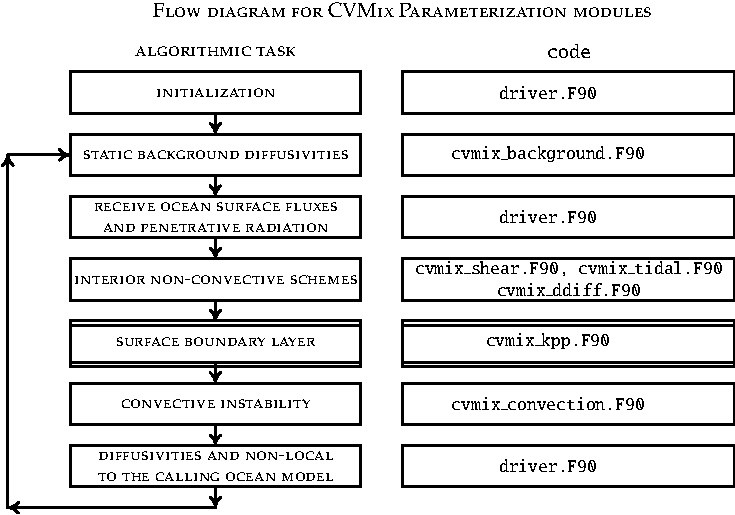
\includegraphics[angle=0,width=15cm,bb=0 0 353 247]{./mfpic_figs/cvmix_flow_diagram.pdf}
\caption[Flow diagram for CVMix schemes]{\sf This flow diagram depicts
  the general algorithmic steps required to utilize the CVMix
  parameterization modules.  The initialization step occurs in one of
  the CVMix drivers that exercises a chosen mixing scheme {\tt
    driver.F90} if running CVMix code as a stand-alone one-dimensional
  model.  Otherwise it occurs via the ocean model if running CVMix
  modules as part of an ocean model such as MPAS-ocean, MOM, or POP.
  This initialization serves to set up arrays and derived type
  structures, all as a function of the input that it receives from the
  calling ocean model code.  The next step during initialization is to
  call the module {\tt CVmix\_background.F90} to fill chosen static
  background diffusivities.  Upon entering the time dependent portion
  of the ocean model integration, the driver receives surface fluxes
  and penetrative radiative fluxes.  Calls are made to chosen interior
  non-convective mixing schemes, such as shear mixing, tide mixing,
  and double diffusion.  Thereafter, the surface boundary layer scheme
  is called, with KPP the scheme targetted for CVMix.  The boundary
  layer calculation is key to the whole process, as it must come after
  the interior non-convective portion, and before the convective
  portion.  After the boundary layer, then convective mixing is
  called, with regions of gravitationally unstable water given a large
  diffusivity.  Notably, if KPP is used for the surface boundary
  layer, convective mixing is performed only beneath the KPP boundary
  layer.  The final step returns the diffusivity $K_{\lambda}$,
  viscosity, and non-local transport $\gamma_{\lambda}$, arrays to the
  calling ocean model code.  A new time step starts by reinitializing
  the diffusivities to their static background values.}
\label{fig:vertical_mix_flow_cvmix}
\end{center}
\end{figure}
%%%%%%%%%%%%%%%%%%%%%%%%%%%%%%%%%%%%%%%%%%%%%%%%%%%%%%%%%%%%%%%%%%%%%%%%



